%PID Controller Closed Loop Diagram.
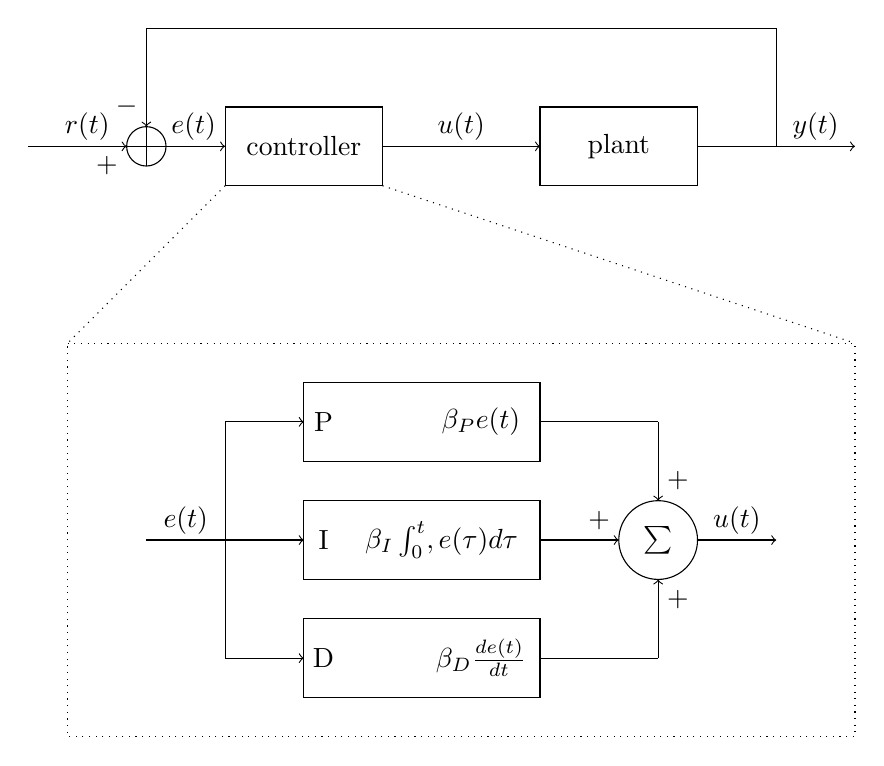
\begin{tikzpicture} 
  \draw (3,1) -- (1,1) -- (1,2) -- (3,2) -- cycle;
  \draw [->] (3,1.5) -- (5,1.5);
  \draw (7,1) -- (5,1) -- (5,2) -- (7,2) -- cycle;
  \draw [->] (7,1.5) -- (9,1.5);
  \draw (8,1.5) -- (8,3) -- (0,3);
  \draw [->] (0,3) -- (0,1.75);
  \draw (0,1.5) circle [radius=0.25];
  \draw (0,1.75) -- (0,1.25);
  \draw (-0.25, 1.5) -- (0.25, 1.5);
  \draw [->] (0.25,1.5) -- (1,1.5);
  \draw [->] (-1.5,1.5) -- (-0.25, 1.5);
  \draw (0.6,1.75) node {$e(t)$};
  \draw (-0.75,1.75) node {$r(t)$};
  \draw (4,1.75) node {$u(t)$};
  \draw (8.5,1.75) node {$y(t)$};
  \draw (2, 1.5) node {controller};
  \draw (6, 1.5) node {plant};
  \draw (-0.25,2) node {$-$};
  \draw (-0.5,1.25) node {$+$};
  
  \draw [dotted] (1, 1) -- (-1, -1);
  \draw [dotted] (3, 1) -- (9, -1);
  \draw [dotted] (-1,-1) -- (9,-1) -- (9,-6) -- (-1,-6) -- cycle;
  \draw (0,-3.5) -- (1,-3.5);
  \draw (1,-5) -- (1,-2);
  \draw [->] (1,-3.5) -- (2,-3.5);
  \draw [->] (1,-2) -- (2,-2);
  \draw [->] (1,-5) -- (2,-5);
  \draw (2, -1.5) -- (5, -1.5) -- (5, -2.5) -- (2, -2.5) -- cycle;
  \draw (2, -3) -- (5, -3) -- (5, -4) -- (2, -4) -- cycle; 
  \draw (2, -4.5) -- (5, -4.5) -- (5, -5.5) -- (2, -5.5) -- cycle;
  \draw (2.25,-3.5) node {I};
  \draw (3.75,-3.5) node {$\beta_I\int_0^t, e(\tau) d\tau$};
  \draw (4.25,-2) node {$\beta_P e(t) $};
  \draw (2.25,-2) node {P};
  \draw (2.25,-5) node {D};
  \draw (4.25,-5) node {$\beta_{D} \frac{de(t)}{dt}$};
  \draw (5, -5) -- (6.5,-5);
  \draw (5, -2) -- (6.5,-2);
  \draw [->] (6.5,-2) -- (6.5, -3);
  \draw [->] (6.5,-5) -- (6.5, -4);
  \draw [->] (5, -3.5) -- (6,-3.5);
  \draw (6.5, -3.5) circle [radius=0.5];
  \draw (6.5, -3.5) node {$\sum$};
  \draw [->] (7,-3.5) -- (8, -3.5);
  \draw (0.5,-3.25) node {$e(t)$};
  \draw (7.5,-3.25) node {$u(t)$};
  \draw (6.75,-2.75) node {$+$};
  \draw (6.75,-4.25) node {$+$};
  \draw (5.75,-3.25) node {$+$};
\end{tikzpicture}

